
\documentclass[preprint,12pt]{elsarticle}
\usepackage{algorithm}
\usepackage{algpseudocode}
\usepackage{amssymb}
\usepackage{amsmath}
\usepackage{tikz}
\usetikzlibrary{arrows.meta,positioning,fit,calc}
\usepackage{graphicx}
\usepackage{subfig}
\usepackage{booktabs}
\usepackage{tabularx}
\usepackage{longtable}
\usepackage{float} % for [H]
\usepackage{placeins}
\usepackage[margin=1in]{geometry}
\usepackage{url}
\usepackage{hyperref}
\usepackage[utf8]{inputenc}
% Helpful macros (optional)
\newcommand{\Cat}{\mathrm{Cat}}
\newcommand{\softmax}{\mathrm{softmax}}
\newcommand{\onehot}{\mathrm{onehot}}
\usepackage{textcomp}
\DeclareUnicodeCharacter{2212}{-}
\journal{Decision Analytics Journal}


\begin{document}

\begin{frontmatter}

\title{Sample-Efficient Adaptive Mock Interview System using Model-Based Reinforcement Learning}

\author[inst1]{Shilpa Kadam}
\affiliation[inst1]{organization={Department of Mathematics, BITS Pilani, Hyderabad Campus},
            city={Hyderabad},
            state={Telangana},
            country={India}}

\author[inst2]{Snehanshu Banerjee}
\affiliation[inst2]{organization={BITS Pilani, Hyderabad Campus},
            city={Hyderabad},
            state={Telangana},
            country={India}}

\author[inst3]{Jabez Christopher}
\affiliation[inst3]{organization={Department of Computer Science and Information Systems, BITS Pilani, Hyderabad Campus},
            city={Hyderabad},
            state={Telangana},
            country={India}}

\author[inst1]{P. T. V. Praveen Kumar}

\author[inst1]{Dipak K. Satpathi}

\begin{abstract}
Adaptive learning platforms can improve mock-interview preparation by adapting question difficulty and recommending targeted learning content. However, learning effective policies is challenging under limited interaction budgets and large discrete action spaces. We present a reinforcement learning framework for adaptive mock interviews that selects question difficulty and learning outcomes and recommends multi-modal content based on learner state. Using a simulated environment with tagged learning outcomes, question banks, and content modalities, we compare five controllers: a rule-based heuristic, Deep Q-Network (DQN with prioritized replay), Proximal Policy Optimization (PPO), Probabilistic Ensembles with Trajectory Sampling (PETS), and Model-Based Policy Optimization (MBPO) adapted to factorized discrete actions.
Results show that PPO achieves strong reward-aligned performance with favorable compute cost, while DQN provides competitive returns with higher training time. Among model-based methods, PETS demonstrates stable learning with planning-driven improvements but higher compute overhead, whereas MBPO reduces average time-to-mastery but exhibits sensitivity across random seeds and weaker reward-aligned performance under the current reward specification. We report learning curves, time-to-mastery, post-content gains by modality, calibration of mastery estimates for model-based methods, stability across seeds, and compute–reward trade-offs. These findings highlight practical trade-offs between pedagogical efficiency, stability, and deployment cost when applying model-free versus model-based RL to adaptive learning.
\end{abstract}

\begin{keyword}
Model-Based Reinforcement Learning \sep PETS \sep MBPO \sep Adaptive Assessment \sep Personalized Learning \sep Intelligent Tutoring System \sep Learning Outcomes \sep Content Recommendation \sep Data Science Education \sep Educational Simulation \sep IRT-based Question Modeling \sep Off-Policy Evaluation
%% MSC codes here, in the form: \MSC code \sep code
%% or \MSC[2008] code \sep code (2000 is the default)
\end{keyword}

\end{frontmatter}
\section{Introduction}

In recent years, the adoption of Artificial Intelligence (AI) and Reinforcement Learning (RL) techniques in education has transformed how learners interact with digital platforms. However, educational institutions and online learning platforms face a critical operational challenge: how to make sequential pedagogical decisions at scale-deciding not just whether a learner is ready for the next topic, but \textit{when}, \textit{how}, and \textit{through which content modality} they should progress. Adaptive learning systems are increasingly being used to personalize content delivery, assess learner proficiency, and enhance engagement, yet most existing systems rely on static rule-based logic or supervised learning models that lack the sequential decision-making capability essential for this complex optimization problem. 

A deep learning-based mock interview system was developed that provided real-time feedback on facial expressions, speech rate, and grammar to improve interview readiness. While effective in personalized feedback generation, their approach was primarily rule-based; they lacked sequential decision-making to dynamically tailor future practice sessions. Also, it failed to capture the temporal dependencies between successive learning actions, such as how a learner's response to one question should influence the next question or recommended study material ~\cite{Patil2021}. A Generative Adversarial Network (GAN) was integrated into a virtual job interview training system to detect behavioral weaknesses and generate personalized feedback for users. Their mixed-methods study showed that GAN-based behavioral insights enhanced participants' perceived interview performance ~\cite{Heimerl2022}. A goal-directed design theory was implemented to improve the user experience and interaction design of AI-based mock interview systems for graduates. It emphasized understanding user goals and proposing design strategies that enhance engagement and usability ~\cite{Miao2020}. In contrast, this work treats the educational tutoring task as a \textbf{sequential decision problem} and proposes a reinforcement learning-based Intelligent Decision Support System (IDSS) where platform decisions (content selection, difficulty calibration) evolve dynamically based on continuous learner feedback rather than predefined interaction rules.

In long-duration programs such as the six-month program on data science courses, learners often face difficulties in revising fundamental concepts while preparing for interviews. Traditional mock tests provide assessment but lack contextual feedback and content-level guidance. Learners who answer incorrectly must manually search for relevant material, leading to cognitive overload and inefficient revision. Educational platform designers must resolve compounding uncertainties: Which learner is confused about which concept? What content modality will best resolve that confusion? How much difficulty increase is pedagogically safe without causing disengagement? There is therefore a need for intelligent decision-making systems that can automatically and adaptively select the optimal pedagogical intervention (test difficulty, content type) in real time, measure concept mastery progression, and reduce manual instructor oversight—ultimately improving learning outcomes while reducing operational burden on educators.

To address this gap, in this paper we propose an Adaptive Mock Interview System framed as a Decision Support System (DSS) powered by Model-Based Reinforcement Learning (MBRL). The system operationalizes the educational decision problem as a Markov Decision Process (MDP), where the state encodes learner mastery profiles, available actions are pedagogical interventions (question difficulty $\times$ content modality combinations), and the reward function balances learning progress against engagement metrics. Unlike model-free RL approaches that learn purely from interaction data, MBRL explicitly models the environment's dynamics (how learner knowledge evolves given an intervention) to achieve higher sample efficiency—an essential requirement in education, where data from each learner is limited, exploration must remain pedagogically safe, and real-time deployment requires rapid convergence. We evaluate two state-of-the-art MBRL algorithms, Probabilistic Ensembles with Trajectory Sampling (PETS) ~\cite{chua2018pets} and Model-Based Policy Optimization (MBPO) ~\cite{janner2019mbpo}, on a simulated educational environment designed to reflect the progression of learners through outcomes-based assessments in addition to DQN and PPO. These algorithms enable the system to plan ahead anticipating how learners will respond to different interventions rather than simply reacting to past performance.

The proposed IDSS automatically optimizes two critical decision variables: (1) question difficulty, adjusted based on real-time mastery probability estimation, and (2) content recommendation, suggesting the most relevant learning material (e.g., videos, slides, handouts) whenever the learner demonstrates knowledge gaps. The underlying decision policy's objective is to maximize cumulative mastery gain while minimizing learner frustration—a multi-objective optimization quantified through reward shaping derived from correctness, response time, and post-content performance improvements. This formulation ensures the IDSS not only improves learning outcomes but also respects learner well-being, a critical consideration for platform stakeholders. To ensure result reliability and decision robustness, we conducted multiple simulation runs, confirming the consistency of model convergence, reward trajectories, and mastery trends across randomized initializations. The entire setup, including simulator, data schema, and evaluation dashboards, has been developed as a reproducible experimental framework for educational decision analytics research, enabling educators and platform developers to validate and deploy the IDSS in their own contexts.

\section{Related Work}
Adaptive learning systems have long sought to tailor instruction to individual learners. Early approaches employed Bayesian Knowledge Tracing (BKT)~\cite{xu2012bkt} and Item Response Theory (IRT)~\cite{lord1980irt} to estimate learner proficiency and adapt question difficulty. With advances in deep learning, Deep Knowledge Tracing (DKT)~\cite{piech2015dkt} and Dynamic Key-Value Memory Networks~\cite{zhang2017dkt}, ~\cite{Minn2018} and ~\cite{Liu2022} improved the accuracy of knowledge state estimation. These methods primarily focus on prediction rather than sequential decision-making.

Reinforcement Learning (RL) has gained prominence in educational technology due to its ability to optimize long-term learning outcomes. Model-free methods such as Q-learning and Deep Q-Networks (DQN) have been applied to content sequencing and hint generation~\cite{doroudi2019adaptive}, while policy-gradient approaches have been explored for curriculum optimization~\cite{rafferty2016active}. Nonetheless, model-free algorithms often require extensive interaction data and are sample-inefficient for educational contexts where exploration cannot risk learner experience. On the other hand, model-based RL (MBRL) offers a promising alternative by learning an explicit model of environment dynamics. The PETS algorithm~\cite{chua2018pets} uses probabilistic ensembles and trajectory sampling to plan actions with uncertainty estimation, achieving strong sample efficiency. Similarly, MBPO~\cite{janner2019mbpo} combines short model rollouts with model-free policy updates, balancing model bias and stability. Both methods have demonstrated success in continuous control and robotics domains, but their application in education remains limited.

Recent reviews~\cite{riedmann2025review,moerland2023survey} highlight the growing interest in using RL for personalized learning, particularly in tutoring systems, question selection, and adaptive feedback generation. Prior studies ~\cite{henderson2018matters} and ~\cite{agarwal2021consistency} emphasize the importance of reproducibility and robustness in RL experiments due to their sensitivity to random seeds, data noise, and environment stochasticity. Following these principles, our study performs repeated simulations and variance analysis to ensure the stability and consistency of learning performance. This work thus contributes to the emerging field of educational reinforcement learning by offering a comparative analysis of PETS and MBPO under realistic test blueprints and robustness conditions, aligned with outcome-based curricula.

\section{Problem Formulation}

\subsection{Mathematical Representation of Adaptive Learning as an MDP}
The adaptive mock interview and content recommendation system can be modeled as a finite-horizon Markov Decision Process (MDP) defined by the tuple 
\[
\mathcal{M} = \langle \mathcal{S}, \mathcal{A}, \mathcal{P}, \mathcal{R}, \gamma \rangle,
\]
where:
\begin{itemize}
    \item $\mathcal{S}$ is the \textbf{state space} representing the learner’s knowledge and engagement context,
    \item $\mathcal{A}$ is the \textbf{action space} consisting of available pedagogical interventions,
    \item $\mathcal{P}(s'|s,a)$ is the \textbf{transition probability} capturing the dynamics of learner knowledge update,
    \item $\mathcal{R}(s,a)$ is the \textbf{reward function} quantifying learning progress and engagement, and
    \item $\gamma \in [0,1]$ is the \textbf{discount factor} controlling the importance of future rewards.
\end{itemize}

At each discrete timestep $t$, the learner–agent pair interacts as follows:
\[
s_t \in \mathcal{S}, \quad a_t \in \mathcal{A}, \quad r_t = \mathcal{R}(s_t, a_t), \quad s_{t+1} \sim \mathcal{P}(s_{t+1} | s_t, a_t).
\]
The objective of the reinforcement learning agent is to learn a policy $\pi_\theta(a|s)$ parameterized by $\theta$ that maximizes the expected cumulative reward:
\[
J(\pi_\theta) = \mathbb{E}_{\pi_\theta}\Bigg[\sum_{t=0}^{T} \gamma^t r_t\Bigg].
\]

\subsection{Mapping MDP Components to the Learning Environment}
In the context of adaptive mock-interviews and content recommendation:
\begin{itemize}
    \item \textbf{State ($s_t$)} — represents the learner’s current mastery profile and engagement level:
    \[
    s_t = [m_1^t, m_2^t, \dots, m_K^t, f_t, \tau_t],
    \]
    where $m_i^t \in [0,1]$ denotes mastery over Learning Outcome $i$, $f_t$ is the current frustration level, and $\tau_t$ is the recent response time.  
    States are updated after each question attempt or content interaction using IRT-informed knowledge tracing.

    \item \textbf{Action ($a_t$)} — includes two disjoint subspaces:
    \[
    \mathcal{A} = \mathcal{A}_Q \cup \mathcal{A}_C,
    \]
    where $\mathcal{A}_Q$ represents the choice of question (LO–difficulty pair) and $\mathcal{A}_C$ denotes the choice of content (modality–topic pair) to recommend.  
    The action determines whether the learner receives another question or is directed to study content before resuming.

    \item \textbf{Transition ($\mathcal{P}$)} — defines how learner mastery evolves given an action:
    \[
    m_i^{t+1} = m_i^t + \eta \cdot \phi(a_t, r_t, \text{content\_type}),
    \]
    where $\eta$ is the learning rate and $\phi$ captures content efficacy (derived empirically from post-content gain statistics).  
    The transition model embodies stochastic learning—mastery can improve, stagnate, or decay depending on engagement and difficulty.

    \item \textbf{Reward ($r_t$)} — encodes pedagogical desirability:
    \[
    r_t = \alpha \cdot \text{correct}_t + \beta \cdot \Delta m_t - \gamma \cdot f_t,
    \]
    where $\text{correct}_t$ is 1 if the learner answers correctly, $\Delta m_t$ is the mastery increment, and $f_t$ is the frustration penalty.  
    The shaping weights $(\alpha, \beta, \gamma)$ balance accuracy, improvement, and well-being.

    \item \textbf{Policy ($\pi_\theta$)} — determines the optimal next pedagogical action based on the learner state:
    \[
    a_t \sim \pi_\theta(a|s_t) = \arg\max_{a \in \mathcal{A}} Q^\pi(s_t, a),
    \]
    where $Q^\pi(s,a)$ represents the expected future return given current state–action.
\end{itemize}
\subsection{Model-Free RL Baselines: DQN and PPO}
\label{subsec:dqn_ppo}


\section{Problem Formulation}
\label{sec:problem_formulation}

\subsection{Mathematical Representation of Adaptive Learning as an MDP}
\label{subsec:mdp_formulation}
The adaptive mock-interview and content recommendation system is modeled as a finite-horizon Markov Decision Process (MDP) defined by
\[
\mathcal{M}=\langle \mathcal{S},\mathcal{A},\mathcal{P},\mathcal{R},\gamma\rangle,
\]
where $\mathcal{S}$ is the state space, $\mathcal{A}$ is the action space, $\mathcal{P}(s'|s,a)$ is the transition kernel, $\mathcal{R}(s,a)$ is the reward function, and $\gamma\in[0,1]$ is the discount factor.
At each timestep $t$,
\[
s_t\in\mathcal{S},\quad a_t\in\mathcal{A},\quad r_t=\mathcal{R}(s_t,a_t),\quad s_{t+1}\sim \mathcal{P}(\cdot\mid s_t,a_t).
\]
The objective is to learn a policy that maximizes expected discounted return over an episode of length at most $T$:
\[
J(\pi)=\mathbb{E}_{\pi}\Bigg[\sum_{t=0}^{T-1}\gamma^t r_t\Bigg].
\]

\subsection{Mapping MDP Components to the Learning Environment}
\label{subsec:mdp_mapping}
In the context of adaptive mock-interviews and content recommendation:

\begin{itemize}
    \item \textbf{State ($s_t$).}
    The state represents the learner's current mastery profile and engagement context:
    \[
    s_t=\big[m_1^t,m_2^t,\dots,m_K^t,\ f_t,\ \tau_t\big],
    \]
    where $m_i^t\in[0,1]$ denotes mastery over Learning Outcome (LO) $i$, $f_t$ is a frustration/engagement indicator, and $\tau_t$ is recent response time.
    \textit{Markov property:} engagement variables $f_t$ and $\tau_t$ are explicitly included in the state so that the simulator updates them from $(s_t,a_t)$, preserving the Markov assumption.

    \item \textbf{Action ($a_t$): gated discrete intervention.}
    The agent chooses either (i) a question intervention or (ii) a content recommendation. We use a \emph{gated} discrete action representation:
    \[
    a_t=(\kappa_t, a_t^{(\kappa)}),\qquad \kappa_t\in\{Q,C\},
    \]
    where $Q$ denotes a question action and $C$ denotes a content action. Conditioned on $\kappa_t$:
    \[
    a_t^{(\kappa)}\in
    \begin{cases}
      \mathcal{A}_Q & \text{if }\kappa_t=Q,\\
      \mathcal{A}_C & \text{if }\kappa_t=C.
    \end{cases}
    \]
    The resulting unified discrete action space is
    \[
    \mathcal{A}=\{(Q,a):a\in\mathcal{A}_Q\}\ \cup\ \{(C,a):a\in\mathcal{A}_C\}.
    \]
    \textit{Implementation note:} this gated representation can be flattened into a single categorical action index, which is directly compatible with DQN and PPO. If masking is used, invalid actions are assigned zero probability under $\pi(\cdot|s)$ (or excluded from $\arg\max$) to ensure only valid interventions are selected.

    \item \textbf{Transition ($\mathcal{P}$).}
    The transition kernel specifies how mastery and engagement evolve given an action:
    \[
    m_i^{t+1}=m_i^t+\eta\cdot \phi(a_t,r_t,\text{content\_type}) + \xi_i^t,
    \]
    where $\eta$ is a learning rate, $\phi(\cdot)$ captures content efficacy (derived from post-content gain statistics), and $\xi_i^t$ denotes stochastic variability in learning.
    Engagement variables $(f_t,\tau_t)$ are also updated by the simulator as stochastic/deterministic functions of $(s_t,a_t)$.
    \textit{Simulator stochasticity:} the simulator captures randomness in correctness, mastery updates, and engagement dynamics through the noise terms (e.g., $\xi_i^t$) and stochastic response modeling inside $\mathcal{P}(s'|s,a)$.

    \item \textbf{Reward ($r_t$).}
    The reward encodes pedagogical desirability:
    \[
    r_t=\alpha\cdot \mathrm{correct}_t + \beta\cdot \Delta m_t - \gamma_f\cdot f_t,
    \]
    where $\mathrm{correct}_t\in\{0,1\}$ indicates whether the learner answered correctly, $\Delta m_t$ is the mastery increment, and $f_t$ is a frustration penalty. The weights $(\alpha,\beta,\gamma_f)$ balance accuracy, improvement, and well-being.

    \item \textbf{Episode termination and horizon.}
    An episode corresponds to a mock-interview session of at most $T$ decisions. Episodes terminate when either (i) a mastery criterion is reached (e.g., target LO mastery exceeds a threshold) or (ii) the step budget $T$ is exhausted. Terminal transitions are handled by setting the next-state value to zero in bootstrapped targets.

    \item \textbf{Policy ($\pi$): reviewer-proof definition.}
    For value-based methods, the policy is greedy with respect to the learned action-value function:
    \[
    \pi_{\text{greedy}}(s)=\arg\max_{a\in\mathcal{A}} Q_\phi(s,a),
    \]
    with $\epsilon$-greedy exploration during training. For policy-gradient methods, actions are sampled from a stochastic categorical policy:
    \[
    a_t\sim \pi_\theta(\cdot|s_t), \qquad \pi_\theta(\cdot|s_t)\ \text{categorical over } \mathcal{A}.
    \]
\end{itemize}

% ==========================================================
% Model-free baselines aligned to the above MDP
% ==========================================================
\subsection{Model-Free Baselines in the Discrete Gated Action Space}
\label{subsec:model_free_alignment}

\subsubsection{DQN with Prioritized Replay (PER)}
\label{subsubsec:dqn_per}
Deep Q-Network (DQN) learns an approximation to the optimal action-value function $Q^\ast(s,a)$ using a neural network $Q_\phi(s,a)$ and a target network $Q_{\bar\phi}$. The one-step TD loss is
\[
\mathcal{L}_{\text{DQN}}(\phi)=
\mathbb{E}_{(s,a,r,s')\sim \mathcal{D}}
\Big[
w_i\big(r+\gamma(1-\mathbf{1}_{\text{term}})\max_{a'}Q_{\bar\phi}(s',a')-Q_\phi(s,a)\big)^2
\Big],
\]
where $\mathcal{D}$ is the replay buffer, and $\mathbf{1}_{\text{term}}$ indicates episode termination (set to $1$ for terminal transitions).
We use \emph{Prioritized Experience Replay (PER)}: samples are drawn with probability proportional to $|\delta_i|^{\alpha_{\text{PER}}}$ and reweighted by $w_i=(N\cdot p_i)^{-\beta_{\text{PER}}}$ to reduce bias.

\paragraph{Action selection (discrete gated actions).}
During training, DQN uses $\epsilon$-greedy exploration:
\[
a_t=
\begin{cases}
\arg\max_{a\in\mathcal{A}} Q_\phi(s_t,a), & \text{with prob. } 1-\epsilon,\\
\text{Uniform}(\mathcal{A}), & \text{with prob. } \epsilon,
\end{cases}
\]
with $\epsilon$ annealed over steps. In our environment, the gated discrete action space $\mathcal{A}$ can be flattened to a single discrete index (question or content), enabling direct use of DQN without any discretization of continuous actions.

\paragraph{Episode termination and simulator stochasticity.}
Episodes terminate at mastery attainment or at the horizon $T$. The simulator stochastically generates correctness outcomes and mastery/engagement updates through $\mathcal{P}(s'|s,a)$, ensuring the replay buffer contains transitions that reflect both pedagogical effects and variability across learners.

\subsubsection{Proximal Policy Optimization (PPO, discrete)}
\label{subsubsec:ppo_discrete}
PPO optimizes a stochastic categorical policy $\pi_\theta(a|s)$ over the unified discrete action space $\mathcal{A}$ together with a value function $V_\nu(s)$ using the clipped surrogate objective:
\[
\max_{\theta}\ \mathbb{E}\Big[
\min\big(r_t(\theta)\hat{A}_t,\ \mathrm{clip}(r_t(\theta),1-\epsilon,1+\epsilon)\hat{A}_t\big)
\Big]
-\lambda_V\big(V_\nu(s_t)-\hat{R}_t\big)^2
+\lambda_H \mathcal{H}[\pi_\theta(\cdot|s_t)],
\]
where $r_t(\theta)=\frac{\pi_\theta(a_t|s_t)}{\pi_{\theta_{\text{old}}}(a_t|s_t)}$, $\hat{A}_t$ is the (GAE) advantage estimate, $\hat{R}_t$ is the return-to-go, $\epsilon$ is the clip range, and $\mathcal{H}$ is the entropy bonus.

\paragraph{Episode termination consistency.}
Rollouts are collected within episodes that terminate at mastery attainment or at horizon $T$. Returns and advantage estimates treat terminal states by stopping bootstrapping at termination (i.e., the value of terminal next states is set to zero), ensuring PPO updates are consistent with the finite-horizon MDP.

\paragraph{Large discrete action spaces.}
PPO updates on mini-batches from short on-policy rollouts, and the entropy bonus $\lambda_H \mathcal{H}[\pi_\theta(\cdot|s)]$ encourages exploration, which is particularly useful in large discrete action spaces induced by the gated tutoring interventions.


\subsubsection*{Similarities and Differences (DQN vs PPO)}
\begin{itemize}
  \item \textbf{Common ground.} Both are model-free and interact with the same MDP, state, actions, and reward. Both can respect blueprint constraints (difficulty mix) by masking or reward penalties.
  \item \textbf{Policy form.} DQN is \emph{value-based} with implicit (greedy/$\epsilon$-greedy) policy; PPO learns an explicit \emph{stochastic} policy over discrete actions with a learned value baseline.
  \item \textbf{Exploration.} DQN relies on $\epsilon$-greedy; PPO explores via its categorical action distribution with entropy regularization (often smoother exploration for multi-action pedagogical choices).
  \item \textbf{Stability.} PPO’s clipped objective usually reduces training oscillations; DQN benefits from target networks and PER but can still show higher variance in sparse/imperfectly shaped rewards.
  \item \textbf{Sample use.} DQN reuses replay data extensively; PPO’s on-policy batches are fresher but less reused. In our setting, PPO’s stability often offsets lower reuse when reward shaping is modest.
  \item \textbf{When each shines.} 
  DQN is strong when Q-targets are well-shaped and action gaps are clear (e.g., strong signal that “content vs question” choices differ).
  PPO is preferable when we need calibrated stochastic choice among comparable actions (e.g., choosing modality or difficulty under uncertainty) and when variance reduction is critical for lesson pacing.
\end{itemize}

\subsubsection*{How DQN/PPO Compare to PETS/MBPO}
\begin{itemize}
  \item \textbf{Sample-efficiency.} PETS and MBPO reduce interaction cost by planning or short model rollouts; in our simulator, they typically reach target reward/time-to-mastery with fewer steps than DQN/PPO.
  \item \textbf{Early learning.} PETS often achieves strong early returns due to ensemble planning; PPO tends to start more stable than DQN. MBPO surpasses both DQN/PPO at moderate budgets via model-augmented updates.
  \item \textbf{Variance.} PPO $<$ DQN in variance; MBPO is usually the most stable across seeds when the learned dynamics are reasonable.
\end{itemize}

\subsubsection{Empirical Insights on Our Simulated Data}
We trained each baseline on identical seeds and budgets (paired design; $S$ seeds). We report mean$\pm$SD and 95\% CIs and test DQN vs PPO with paired $t$-test (or Wilcoxon when normality failed). Across runs, PPO showed (i) faster early improvement and (ii) lower variance; DQN sometimes matched PPO’s final return with more steps when the reward was strongly shaped by correctness and post-content gains.

\begin{table}[!t]
\centering
\caption{DQN vs PPO on the simulated education MDP}
\label{tab:dqn_ppo_perf}
\begin{tabular}{lccc}
\hline
\textbf{Metric} & \textbf{DQN (PER)} & \textbf{PPO} & \textbf{Sig. test} \\
\hline
AUC (reward) @10k steps & \textit{DQN\_AUC10k} & \textit{PPO\_AUC10k} & \textit{$p$-value} \\
Time-to-Mastery (steps) & \textit{DQN\_TTM} & \textit{PPO\_TTM} & \textit{$p$-value} \\
Final Return @30k steps & \textit{DQN\_R30k} & \textit{PPO\_R30k} & \textit{$p$-value} \\
Reward Variance (seeds) & \textit{DQN\_Var} & \textit{PPO\_Var} & --- \\
Compute (wall-clock, s)  & \textit{DQN\_Time} & \textit{PPO\_Time} & --- \\
\hline
\end{tabular}
\vspace{-2mm}
\end{table}

\paragraph{Takeaways.} 
PPO is generally the better \emph{model-free} controller for this domain because it is more stable, explores more gracefully over similarly good pedagogical actions, and achieves better or equal sample-efficiency at small to medium budgets. DQN remains competitive when rewards are strongly shaped and when extensive replay offers value—yet it typically needs more steps to match PPO’s performance. Both are outperformed in data-efficiency by MBPO and, during early learning, by PETS.

\subsubsection{Practical Guidance for Deployment}
If live data are scarce or expensive, prefer MBPO (overall) or PETS (fast start). If you must stay model-free for simplicity or compute:
use PPO for stable improvement and predictable pacing; retain DQN (with PER) when compute is tight and you can afford more samples and stronger reward shaping.

\subsection{Model-Based Reinforcement Learning Instantiation}
In a model-based approach, the transition dynamics $\mathcal{P}$ are not fixed but learned from interaction data to predict next states and rewards.  
Let $\hat{\mathcal{P}}_\psi(s',r|s,a)$ denote the learned model with parameters $\psi$.  
The model is trained to minimize prediction error:
\[
\min_\psi \mathbb{E}_{(s,a,s',r)\sim \mathcal{D}} \Big[ \|s' - \hat{s}'_\psi(s,a)\|^2 + (r - \hat{r}_\psi(s,a))^2 \Big].
\]

\subsubsection{PETS Formulation}

\paragraph{Action factorization.}
We model the tutoring action as multi-discrete and factorized:
\begin{equation}
a_t = (d_t,\ell_t,m_t), \qquad
\pi(a_t \mid s_t) = \pi_d(d_t \mid s_t)\,\pi_\ell(\ell_t \mid s_t)\,\pi_m(m_t \mid s_t).
\label{eq:pets_action_factorization}
\end{equation}
For planning, we maintain per-timestep categorical logits for each action component,
\begin{equation}
\left\{\phi^{(d)}_h,\;\phi^{(\ell)}_h,\;\phi^{(m)}_h\right\}_{h=0}^{H-1}.
\label{eq:pets_logits}
\end{equation}

\paragraph{Sampling candidate sequences (discrete CEM).}
At each environment step $t$, PETS performs MPC by optimizing a length-$H$ action sequence using the cross-entropy method (CEM) over discrete actions. For each CEM iteration, we sample $N$ candidate sequences by independently sampling each component at each horizon step:
\begin{align}
d^{(n)}_{t+h} &\sim \Cat\!\left(\softmax\!\left(\phi^{(d)}_{h}\right)\right), \nonumber\\
\ell^{(n)}_{t+h} &\sim \Cat\!\left(\softmax\!\left(\phi^{(\ell)}_{h}\right)\right), \nonumber\\
m^{(n)}_{t+h} &\sim \Cat\!\left(\softmax\!\left(\phi^{(m)}_{h}\right)\right),
\label{eq:pets_sampling}
\end{align}
for $h=0,\dots,H-1$ and $n=1,\dots,N$. Each sampled sequence is rolled out through the learned ensemble dynamics model
$p_{\theta_i}(s' \mid s,a)$ to estimate predicted return (optionally including an uncertainty penalty based on ensemble disagreement).

\paragraph{Elite update (cross-entropy update).}
We select the top $K$ sequences (elites) by predicted return and update the logits using elite frequencies. For example, for the difficulty component at step $h$,
\begin{equation}
\phi^{(d)}_h \leftarrow (1-\eta)\,\phi^{(d)}_h + \eta \cdot \log\!\Big(\mathrm{freq}_{\mathrm{elite}}(d \text{ at } h) + \epsilon\Big),
\label{eq:pets_update}
\end{equation}
and similarly for $\phi^{(\ell)}_h$ and $\phi^{(m)}_h$, where $\eta \in (0,1]$ is the update rate and $\epsilon>0$ is a small smoothing constant.

\paragraph{MPC execution.}
After $J$ CEM iterations, we execute only the first action $(d_t,\ell_t,m_t)$ from the best planned sequence, observe the real next state $s_{t+1}$, append $(s_t,a_t,r_t,s_{t+1})$ to the dataset/replay buffer, and replan at the next step.

\paragraph{Reported hyperparameters.}
We report $H$, $N$, $K$ (or elite fraction), $J$, $\eta$, ensemble size $E$, and the action encoding used by the dynamics model (one-hot vs. embedding).

% ==========================================================
% Algorithm 1: PETS with Factorized Categorical CEM (MPC)
% ==========================================================
\begin{algorithm}[H]
\caption{PETS with Factorized Categorical CEM for Multi-Discrete MPC}
\label{alg:pets_catcem}
\begin{algorithmic}[1]
\Require Dynamics ensemble $\{p_{\theta_i}(s'|s,a)\}_{i=1}^E$, reward $\hat r(s,a)$, horizon $H$, discount $\gamma$
\Require CEM iters $J$, candidates $N$, elites $K$, update rate $\eta$, smoothing $\epsilon$
\For{each environment step $t=0,1,2,\dots$}
    \State $s \gets s_t$
    \State Initialize logits $\{\phi^{(d)}_h,\phi^{(\ell)}_h,\phi^{(m)}_h\}_{h=0}^{H-1}$ (e.g., zeros)
    \For{$j=1$ to $J$}
        \For{$n=1$ to $N$}
            \State $s^{(n)}_0 \gets s$, $\widehat{J}^{(n)} \gets 0$
            \For{$h=0$ to $H-1$}
                \State $d^{(n)}_{h} \sim \mathrm{Cat}(\mathrm{softmax}(\phi^{(d)}_{h}))$
                \State $\ell^{(n)}_{h} \sim \mathrm{Cat}(\mathrm{softmax}(\phi^{(\ell)}_{h}))$
                \State $m^{(n)}_{h} \sim \mathrm{Cat}(\mathrm{softmax}(\phi^{(m)}_{h}))$
                \State $a^{(n)}_{h} \gets (d^{(n)}_{h},\ell^{(n)}_{h},m^{(n)}_{h})$
                \State Sample $i \sim \mathrm{Uniform}\{1,\dots,E\}$ and $s^{(n)}_{h+1} \sim p_{\theta_i}(\cdot|s^{(n)}_h,a^{(n)}_h)$
                \State $\widehat{J}^{(n)} \gets \widehat{J}^{(n)} + \gamma^h \hat r(s^{(n)}_h,a^{(n)}_h)$
            \EndFor
        \EndFor
        \State Let $\mathcal{E}$ be indices of top-$K$ sequences by $\widehat{J}^{(n)}$
        \For{$h=0$ to $H-1$}
            \State $f^{(d)}_h(x) \gets \frac{1}{K}\sum_{n\in\mathcal{E}} \mathbf{1}[d^{(n)}_h=x]$ for all $x\in\mathcal{D}$
            \State $f^{(\ell)}_h(y) \gets \frac{1}{K}\sum_{n\in\mathcal{E}} \mathbf{1}[\ell^{(n)}_h=y]$ for all $y\in\mathcal{L}$
            \State $f^{(m)}_h(z) \gets \frac{1}{K}\sum_{n\in\mathcal{E}} \mathbf{1}[m^{(n)}_h=z]$ for all $z\in\mathcal{M}$
            \State $\phi^{(d)}_h \gets (1-\eta)\phi^{(d)}_h + \eta \log(f^{(d)}_h+\epsilon)$
            \State $\phi^{(\ell)}_h \gets (1-\eta)\phi^{(\ell)}_h + \eta \log(f^{(\ell)}_h+\epsilon)$
            \State $\phi^{(m)}_h \gets (1-\eta)\phi^{(m)}_h + \eta \log(f^{(m)}_h+\epsilon)$
        \EndFor
    \EndFor
    \State $n^\star \gets \arg\max_n \widehat{J}^{(n)}$
    \State Execute $a_t \gets a^{(n^\star)}_{0}$, observe $(r_t,s_{t+1})$, and store $(s_t,a_t,r_t,s_{t+1})$
\EndFor
\end{algorithmic}
\end{algorithm}

\subsubsection{MBPO Formulation}

\paragraph{MBPO structure.}
We follow the standard MBPO structure: (i) collect real transitions and fit/update the ensemble dynamics model; (ii) generate short model rollouts of length $K$ from real states; and (iii) train the policy using a mixture of real and model-generated transitions.

\paragraph{Model rollouts (short horizon).}
We sample starting states $s_0$ from the real replay buffer. For $k=0,\dots,K-1$, we sample a factorized action from the categorical policy:
\begin{equation}
d_k \sim \pi_d(\cdot \mid s_k), \qquad
\ell_k \sim \pi_\ell(\cdot \mid s_k), \qquad
m_k \sim \pi_m(\cdot \mid s_k),
\label{eq:mbpo_factorized_sampling}
\end{equation}
predict the next state using the learned dynamics,
\begin{equation}
s_{k+1} \sim p_{\theta}\!\left(\cdot \mid s_k,\,(d_k,\ell_k,m_k)\right),
\label{eq:mbpo_dynamics_rollout}
\end{equation}
and store the resulting synthetic transition in the model buffer.

\paragraph{Discrete SAC objective (factorized policy).}
The critic learns $Q_{\varphi}(s,a)$ over the joint discrete action $a=(d,\ell,m)$. The actor outputs three categorical distributions $\pi_d$, $\pi_\ell$, and $\pi_m$. The joint log-probability under the factorized policy is
\begin{equation}
\log \pi(a \mid s)=\log \pi_d(d \mid s)+\log \pi_\ell(\ell \mid s)+\log \pi_m(m \mid s).
\label{eq:mbpo_joint_logprob}
\end{equation}
Accordingly, the entropy term decomposes additively:
\begin{equation}
\mathcal{H}(\pi)=\mathcal{H}(\pi_d)+\mathcal{H}(\pi_\ell)+\mathcal{H}(\pi_m),
\label{eq:mbpo_entropy_decomp}
\end{equation}
and is weighted by the temperature parameter $\alpha$ in the entropy-regularized actor-critic updates.

\paragraph{Practical note (enumeration vs. sampling).}
If $|\mathcal{A}|=|\mathcal{D}|\;|\mathcal{L}|\;|\mathcal{M}|$ is small, we compute soft value targets by enumerating all joint actions; otherwise we approximate expectations by sampling joint actions from the factorized policy.

\paragraph{Replay mixing.}
We train using mini-batches that mix real and model transitions with ratio $\rho$ (fraction sampled from the real buffer). We report $\rho$, rollout length $K$, rollout refresh frequency, and model-buffer size.
% ==========================================================
% Algorithm 2: MBPO with Factorized Discrete SAC
% ==========================================================

\begin{algorithm}[H]
\caption{MBPO with Factorized Discrete SAC for Multi-Discrete Tutoring Actions}
\label{alg:mbpo_discrete_sac}
\begin{algorithmic}[1]
\Require Environment $\mathcal{E}$
\Require Dynamics ensemble $\{p_{\theta_i}(s'|s,a)\}_{i=1}^E$
\Require Factorized discrete SAC agent: actor $\pi_\omega(a|s)=\pi_{\omega_d}(d|s)\pi_{\omega_\ell}(\ell|s)\pi_{\omega_m}(m|s)$, critics $Q_{\varphi_1},Q_{\varphi_2}$
\Require Real replay buffer $\mathcal{B}$, model buffer $\mathcal{B}_m$
\Require Rollout length $K$, rollout batch size $M$, mixing ratio $\rho \in [0,1]$
\Require Real collection steps $T_{\text{real}}$, dynamics update steps $U$, policy update steps $G$
\State Initialize $\mathcal{B} \gets \emptyset$, $\mathcal{B}_m \gets \emptyset$
\State Initialize $\theta_1,\dots,\theta_E$, $\omega$, $\varphi_1$, $\varphi_2$ (and temperature $\alpha$ if used)
\For{iteration $t=1,2,\dots$}
    \State \textbf{(1) Collect real experience}
    \For{$e=1$ to $T_{\text{real}}$}
        \State Sample $d \sim \pi_{\omega_d}(\cdot|s)$, $\ell \sim \pi_{\omega_\ell}(\cdot|s)$, $m \sim \pi_{\omega_m}(\cdot|s)$
        \State $a \gets (d,\ell,m)$; execute $a$ in $\mathcal{E}$
        \State Observe reward $r$ and next state $s'$
        \State Store $(s,a,r,s')$ in $\mathcal{B}$; set $s \gets s'$
    \EndFor

    \State \textbf{(2) Update dynamics ensemble on real buffer}
    \For{$u=1$ to $U$}
        \State Sample minibatch $\mathcal{D} \subset \mathcal{B}$
        \For{each model $i=1$ to $E$}
            \State Update $\theta_i$ to minimize supervised loss on $(s,a,s')$ in $\mathcal{D}$
        \EndFor
    \EndFor

    \State \textbf{(3) Generate short model rollouts (synthetic transitions)}
    \For{$midx=1$ to $M$}
        \State Sample start state $s_0$ from $\mathcal{B}$; set $s \gets s_0$
        \For{$k=0$ to $K-1$}
            \State Sample $d \sim \pi_{\omega_d}(\cdot|s)$, $\ell \sim \pi_{\omega_\ell}(\cdot|s)$, $m \sim \pi_{\omega_m}(\cdot|s)$
            \State $a \gets (d,\ell,m)$
            \State Sample $i \sim \mathrm{Uniform}\{1,\dots,E\}$
            \State Predict $s' \sim p_{\theta_i}(\cdot|s,a)$
            \State Compute $\hat r \gets \hat r(s,a)$ \Comment{or model reward if learned}
            \State Store $(s,a,\hat r,s')$ in $\mathcal{B}_m$; set $s \gets s'$
        \EndFor
    \EndFor

    \State \textbf{(4) Policy optimization (Discrete SAC) with mixed replay}
    \For{$g=1$ to $G$}
        \State Sample minibatch $\mathcal{D}_r \subset \mathcal{B}$ and minibatch $\mathcal{D}_m \subset \mathcal{B}_m$
        \State Form training batch $\mathcal{D} \gets$ mix of $\mathcal{D}_r$ and $\mathcal{D}_m$ with fraction $\rho$ from $\mathcal{B}$
        \State Update critics $Q_{\varphi_1},Q_{\varphi_2}$ using soft Bellman targets
        \State Use $\log\pi_\omega(a|s)=\log\pi_{\omega_d}(d|s)+\log\pi_{\omega_\ell}(\ell|s)+\log\pi_{\omega_m}(m|s)$ in the entropy term
        \State Update actor parameters $\omega_d,\omega_\ell,\omega_m$ to maximize expected soft value and entropy
        \State Optionally update temperature $\alpha$ to match target entropy
    \EndFor
\EndFor
\end{algorithmic}
\end{algorithm}

\subsection{Educational Relevance of the Formulation}
Formulating the problem as an MDP enables systematic adaptation of both question difficulty and content type according to each learner’s evolving mastery.  
The policy $\pi_\theta$ corresponds to an intelligent teaching strategy; the reward $r_t$ aligns with learning progress; and the transition model $\hat{\mathcal{P}}$ reflects cognitive dynamics.  
PETS and MBPO differ mainly in how they estimate and utilize this model—PETS performs planning using predictive uncertainty, whereas MBPO leverages short model rollouts to accelerate policy improvement. Although PETS and MBPO are often demonstrated on continuous-control benchmarks, both extend naturally to discrete action spaces by (i) using MPC with categorical (multi-discrete) sampling and CE updates for PETS and (ii) retaining MBPO’s short model-rollout replay augmentation while optimizing a categorical policy via a discrete off-policy learner. Together, these formulations provide a principled mathematical foundation for real-time, personalized content recommendation in data-driven education systems.

\subsection{Conceptual Illustration of the MDP Framework}

\begin{figure*}[!t]
\centering
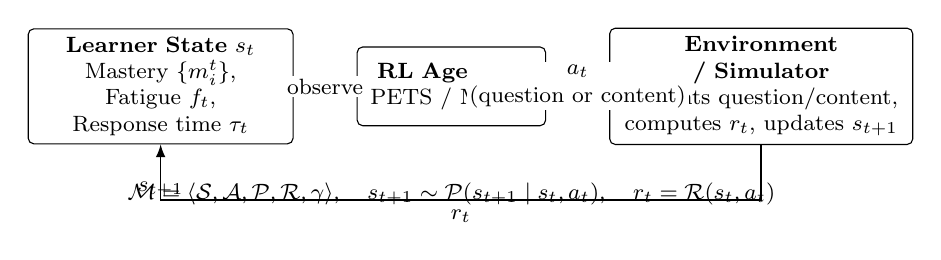
\begin{tikzpicture}[
  font=\footnotesize,
  node distance=8mm,
  >=latex,
  boxA/.style={draw, rounded corners=2pt, align=center, inner sep=3pt,
               text width=0.26\textwidth, minimum height=1.0cm},
  boxB/.style={draw, rounded corners=2pt, align=center, inner sep=3pt,
               text width=0.18\textwidth, minimum height=1.0cm},
  boxC/.style={draw, rounded corners=2pt, align=center, inner sep=3pt,
               text width=0.30\textwidth, minimum height=1.0cm},
  arr/.style={->, line width=0.6pt},
  lbl/.style={midway, fill=white, inner sep=1pt}
]
% Nodes (keep plain ASCII inside text)
\node[boxA] (state) {\textbf{Learner State} $s_t$\\
\footnotesize Mastery $\{m_i^t\}$, Fatigue $f_t$,\\Response time $\tau_t$};

\node[boxB, right=of state] (agent) {\textbf{RL Agent} $\pi_\theta$\\
\footnotesize PETS / MBPO};

\node[boxC, right=of agent] (env) {\textbf{Environment / Simulator}\\
\footnotesize Presents question/content,\\computes $r_t$, updates $s_{t+1}$};

% Arrows
\draw[arr] (state) -- node[lbl]{observe} (agent);
\draw[arr] (agent) -- node[lbl] {\shortstack{$a_t$\\\footnotesize (question or content)}} (env);
\draw[arr] (env.south) |- ++(0,-7mm) -| node[pos=0.25, below] {$r_t$}
                                       node[pos=0.75, below] {$s_{t+1}$} (state.south);

% Compact annotation (pure math, ASCII only)
\node[below=6mm of agent, align=center] {\footnotesize
$\mathcal{M}=\langle\mathcal{S},\mathcal{A},\mathcal{P},\mathcal{R},\gamma\rangle,\quad
s_{t+1}\sim \mathcal{P}(s_{t+1}\mid s_t,a_t),\quad
r_t=\mathcal{R}(s_t,a_t)$};
\end{tikzpicture}
\caption{Conceptual mapping of the RL framework to the adaptive mock-interview process.}
\label{fig:mdp_flow_wide}
\end{figure*}


The conceptual diagram in Fig.~\ref{fig:mdp_flow_wide} illustrates the complete decision loop.  
At each time step $t$, the learner’s internal mastery profile and engagement form the \textbf{state} $s_t$.  
The RL agent observes this state and decides on an \textbf{action} $a_t$—either selecting the next question (difficulty, topic) or recommending a learning resource (video, PPT, article).  
The environment then provides a \textbf{reward} $r_t$, reflecting correctness, engagement, and improvement, and transitions to a new learner state $s_{t+1}$ according to the learned dynamics $\hat{\mathcal{P}}(s_{t+1},r_t|s_t,a_t)$.  

The process continues iteratively, allowing the policy $\pi_\theta$ to adaptively select actions that accelerate mastery and reduce cognitive fatigue.  
This MDP formulation explicitly captures:
\begin{enumerate}
    \item The temporal dependency between successive learning interactions,
    \item The stochastic nature of learner improvement and forgetting,
    \item The trade-off between assessment (questioning) and reinforcement (content recommendation),
    \item The capacity of model-based methods (PETS, MBPO) to plan future trajectories based on predicted outcomes.
\end{enumerate}

Over multiple episodes, the policy converges toward an optimal strategy that balances exploration (testing new question–content combinations) and exploitation (reinforcing known effective interventions).  
This structure directly supports adaptive mastery tracking, personalized pacing, and automated feedback generation for both learners and instructors.

\section{Methodology}

\subsection{System Overview}
The \textbf{Adaptive Mock Interview System} consists of three primary components: 
(1) a Learner Environment Simulator, 
(2) a Model-Based RL Agent, and 
(3) an Instructor Analytics Dashboard. 
Learners are modeled as agents interacting with questions and content linked to predefined Learning Outcomes (LOs). Each LO is tagged with Bloom’s taxonomy level (Recall, Apply, Analyze, etc.) and prerequisite dependencies. The system uses a combination of Item Response Theory (IRT) parameters and Knowledge Tracing (KT) to represent learner ability and predict the probability of answering correctly.

When a learner answers incorrectly, the system either decreases difficulty or recommends the most suitable learning content (video, PPT, or handout). The recommendation trigger is governed by a fail-streak threshold (typically three consecutive incorrect responses). Each content item is associated with a learning outcome and has attributes such as modality, duration, and reading complexity.  

\subsection{Reinforcement Learning Formulation}
The environment is formulated as a Markov Decision Process (MDP):
\begin{itemize}
\item \textbf{State} $(s_t)$: learner mastery vector across all LOs, recent response time, fail-streak count, and content fatigue level.
\item \textbf{Action} $(a_t)$: either (i) question selection (choice of LO and difficulty) or (ii) content recommendation (choice of modality and asset). 
\item \textbf{Reward} $(r_t)$: shaped reward combining correctness (+1), reduced response time (+$\alpha$), and post-content improvement (+$\beta$). Penalties (−$\gamma$) are applied for repeated failures or high frustration.
\item \textbf{Transition} $(s_{t+1})$: governed by the learner model using IRT-based performance updates and stochastic mastery drift.
\end{itemize}

\subsection{Model-Based RL Algorithms}
\subsubsection{PETS}
The PETS algorithm~\cite{chua2018pets} learns an ensemble of probabilistic neural networks to approximate the transition dynamics $p(s_{t+1}, r_t | s_t, a_t)$. It samples trajectories using the Cross-Entropy Method (CEM) to identify the action sequence that maximizes expected cumulative reward while accounting for ensemble uncertainty. This approach allows the agent to plan adaptively under noisy learner states and balance exploration with performance stability.

\subsubsection{MBPO}
The MBPO algorithm~\cite{janner2019mbpo} combines a learned dynamics model with a model-free learner (Soft Actor–Critic). It generates short model rollouts (1–5 steps) from real experience and augments them with model-free updates. This hybrid approach reduces model bias while maintaining sample efficiency. In this system, MBPO is used to optimize both question selection and content recommendation under blueprint constraints.

\paragraph{Episode and horizons.}
One environment step corresponds to one tutoring decision $a_t=(d_t,\ell_t,m_t)$ applied to the learner state $s_t$. An episode is a complete tutoring session of at most $T$ decisions, terminating either when a mastery criterion is met or when $t=T-1$. PETS uses MPC planning horizon $H$, i.e., at each real step $t$ it plans a length-$H$ action sequence under the learned dynamics ensemble but executes only the first action and replans at $t+1$. MBPO uses short model rollout length $K$ to generate synthetic transitions from real states; $K$ is independent of the episode length $T$.

\begin{table}[t]
\centering
\caption{Discrete adaptation of PETS and MBPO for multi-discrete tutoring actions.}
\label{tab:discrete_adaptation}
\begin{tabular}{p{3.4cm} p{5.4cm}}
\toprule
\textbf{Component} &  \textbf{Our adaptation (multi-discrete)} \\
\midrule
Action space &  Multi-discrete: \(a=(d,\ell,m)\) (joint or factorized) \\
PETS planner &  CEM over \textit{categorical} logits; sample discrete sequences; elite-based logit update \\
PETS execution &  Same MPC; first discrete action executed each step \\
Dynamics model &  Same; trained on discrete actions (one-hot / embeddings) \\
Uncertainty handling & Same; optional variance penalty across ensemble rollouts \\
MBPO inner RL & Discrete policy optimizer (categorical actor–critic / discrete SAC variant); entropy regularization preserved \\
MBPO rollouts &  Same; rollout length \(K\) tuned; model buffer mixed with real replay \\
\bottomrule
\end{tabular}
\end{table}



\subsection{Experimental Design and Validation}
This study follows a simulation-based experimental design to evaluate the two model-based reinforcement learning algorithms—PETS and MBPO—under controlled, reproducible conditions in addition to two model-free reinforcement learning algorithms, DQN-PER and PPO. We compare with rule-based pedagogical heuristic that mimics common adaptive-learning logic (mastery-band difficulty progression with remediation triggers) all evaluated under identical interaction budgets and random seeds.
To evaluate the algorithms reproducibly, we designed a simulator mimicking 200 learners, 30 LOs, and 600 questions parameterized by IRT factors (a, b, c). Approximately 180 learning materials are associated with LOs across six modalities (video, PPT, text, blog, article, handout). Each learner’s session includes 80–140 items, producing over 50,000 logged interactions, with event types such as \textit{question\_shown}, \textit{answered}, and \textit{content\_shown}. The dataset supports both offline policy evaluation (via inverse propensity scoring) and online fine-tuning of MBRL policies.

\subsubsection{Rule-based Decision Logic}
Rule-based heuristic (RB): a deterministic pedagogical controller is defined that selects (question vs content) using engagement thresholds and then chooses the lowest-mastery learning outcome with difficulty determined by mastery bands and content modality chosen by fixed rules (e.g., video/PPT for remediation unless frustration is high).
\paragraph{1) Decide intervention type: question vs.\ content.}

We first choose a gate variable $\kappa_t \in \{Q,C\}$ indicating whether to ask a question ($Q$) or recommend content ($C$). Let $f_t$ denote frustration and $\tau_t$ denote response time at step $t$. Define thresholds $f_{\max}$ and $\tau_{\max}$. The rule is:
\[
\kappa_t =
\begin{cases}
C, & \text{if } f_t \ge f_{\max} \;\text{ or }\; \tau_t \ge \tau_{\max},\\[4pt]
Q, & \text{otherwise}.
\end{cases}
\]

\paragraph{2) If $\kappa_t = Q$: pick LO and difficulty.}

Choose the lowest-mastery learning outcome:
\[
\ell_t = \arg \min_i m_i^t,
\]
where $m_i^t \in [0,1]$ is the mastery for LO $i$ at time $t$.

Then choose difficulty based on mastery bands (blueprint-based):
\[
\text{difficulty}(\ell_t) =
\begin{cases}
\text{Easy},   & \text{if } m_{\ell_t}^t < 0.4,\\[4pt]
\text{Medium}, & \text{if } 0.4 \le m_{\ell_t}^t < 0.7,\\[4pt]
\text{Hard},   & \text{if } m_{\ell_t}^t \ge 0.7.
\end{cases}
\]

\paragraph{3) If $\kappa_t = C$: pick modality and topic.}

The topic is chosen as the same lowest-mastery LO:
\[
\text{topic}_t = \ell_t = \arg \min_i m_i^t.
\]

The content modality is chosen as a function of frustration (or fatigue) level:
\[
\text{modality}_t =
\begin{cases}
\text{short text/handout}, & \text{if } f_t \text{ is high},\\[4pt]
\text{video/PPT},          & \text{otherwise},
\end{cases}
\]
where the second case reflects empirical evidence that video and PPT content yield higher post-content gains in this setting.


A simulation-based design allows precise control of confounding variables such as motivation, fatigue, or course duration, ensuring that observed differences in performance originate purely from the learning algorithms rather than human variability.  The simulator integrates behavioral dynamics derived from educational psychology—such as forgetting curves, skill reinforcement, and mastery plateaus—while maintaining computational efficiency.  
Initial learner proficiency levels are drawn from a beta distribution to emulate heterogeneous populations.  
Success probabilities on each question are determined using the logistic IRT model:
\[
P(\text{correct}) = \frac{1}{1+\exp[-a_i(\theta_j - b_i)]},
\]
where $a_i$ and $b_i$ represent question discrimination and difficulty, and $\theta_j$ is the learner’s latent ability at step~$t$.  
Interactions with recommended content trigger mastery updates based on empirically observed improvement factors.

Both PETS and MBPO were trained within the same simulator interface, sharing identical state, action, and reward definitions.  
Hyperparameters (planning horizon, ensemble size, learning rate, discount factor, rollout length) were tuned via grid search over pilot runs.  
To validate reproducibility, each algorithm was executed across $S=5$ independent random seeds using identical initialization (paired design).  
Results are reported as mean~$\pm$~SD and $95\%$ confidence intervals.  
Paired $t$-tests and Wilcoxon signed-rank tests were used for significance analysis, and Cohen’s~$d$ was computed to measure effect size.  
Bootstrap resampling ($1{,}000$ iterations) was used to estimate confidence intervals due to cohort-level variability.  
Seed-aggregated learning curves with shaded $95\%$ confidence intervals demonstrated consistent convergence trends across all stochastic draws.

Although this setup employs simulated data, its structure is pedagogically grounded and directly transferable to real-world learning platforms (e.g., LMS or MOOC systems).  
The simulator's state and reward representations are aligned with observable metrics such as response time, content engagement, and question-level mastery, ensuring smooth adaptation when real learner data becomes available.
\subsection{Rationale for Simulation-Based Evaluation}
Real-world educational data, although ideal, pose multiple challenges for controlled reinforcement learning experiments. Collecting sufficient learner content interaction data requires prolonged deployment periods and consistent learner participation, which are difficult to guarantee in early-stage research. Moreover, privacy regulations and institutional ethics policies restrict access to fine-grained behavioral logs that would be necessary for continuous policy learning.

To overcome these constraints, we developed a high-fidelity simulated environment that captures key cognitive and behavioral features—such as mastery progression, fatigue, and question difficulty adaptation—using Item Response Theory (IRT) and stochastic mastery updates. This design allows us to perform reproducible and statistically controlled experiments across multiple random seeds and RL algorithms under identical conditions. Although simulation abstracts certain human factors such as motivation or attention span, it enables fair, large-scale comparison of policy learning efficiency before live deployment. In future work, this simulation will serve as a pre-training stage for model initialization prior to real learner fine-tuning.

\subsection{Evaluation Metrics}
The following metrics are used:
\begin{itemize}
\item \textbf{Time-to-Mastery}: average steps to reach 0.8 mastery per LO.
\item \textbf{Post-Content Gain}: change in correctness after content recommendation.
\item \textbf{Cumulative Reward}: total reward per learner session.
\item \textbf{Blueprint Adherence}: deviation from the 20\%-60\%-20\% difficulty distribution.
\item \textbf{Policy Stability}: reward variance across episodes.
\end{itemize}

\subsection{Robustness and Statistical Testing}
To ensure that conclusions generalize beyond a single simulation draw, we executed each algorithm with $S$ independent random seeds (default $S=20$). PETS and MBPO were evaluated under identical simulator initializations per seed (paired design). Primary outcomes included Time-to-Mastery, Post-Content Gain, Cumulative Reward, Reward Variance, and Blueprint Deviation.

For each metric we report $\text{mean}\pm\text{SD}$ and 95\% confidence intervals (CIs). Pairwise significance was assessed via a paired $t$-test (with Shapiro–Wilk normality); when normality was violated we used the Wilcoxon signed-rank test. Effect sizes were reported as Cohen’s $d$ (paired) or Cliff’s $\delta$. To assess sensitivity to cohort composition we computed nonparametric bootstrap CIs by resampling learners (1{,}000 resamples) within each seed. Seed-aggregated learning curves are plotted with shaded 95\% CIs. We further performed sensitivity analyses varying reward weights $(\alpha,\beta,\gamma)$, PETS planning horizon $H\in\{5,10\}$, and MBPO rollout length $k\in\{1,3,5\}$. Off-policy estimates (IPS/DR) include bootstrap CIs and effective sample size (ESS).
\subsection{Threats to Validity}
Although the study demonstrates promising results, certain limitations and validity concerns remain that may influence generalization or interpretation.

\subsubsection{Internal Validity}
Internal validity pertains to whether the observed effects can be confidently attributed to the reinforcement learning algorithms rather than experimental artifacts.  
To mitigate this threat, PETS and MBPO were implemented under identical simulator settings, reward functions, and hyperparameter grids.  
All stochastic elements (learner initialization, question sampling, and environment transitions) were controlled through fixed random seeds per trial.  
Despite these precautions, residual bias may arise from model initialization or hyperparameter sensitivity, which future work can address through Bayesian optimization or automated tuning.

\subsubsection{External Validity}
Since the experiments are conducted using simulated data rather than live classroom interactions, generalization to real learners must be interpreted cautiously.  
But, the simulator was parameterized using realistic learning dynamics drawn from Item Response Theory and mastery learning principles.  
Furthermore, the state and reward features (accuracy, response time, content engagement) are directly observable in real Learning Management Systems (LMS), enabling straightforward transfer of the proposed framework to authentic educational settings.

\subsubsection{Construct Validity}
Construct validity examines whether the operational definitions truly capture the intended learning constructs.  
The reward design—combining correctness, improvement, and response efficiency—was formulated in consultation with domain instructors to ensure pedagogical alignment.  
Still, mastery level and frustration proxies are inferred quantities; future integration of multimodal affective indicators (e.g., gaze, tone, pause duration) would improve construct precision.

\subsubsection{Statistical Validity}
Statistical validity concerns the soundness of inference procedures and robustness against random variation.  
This study used $S=20$ independent seeds with paired evaluations and bootstrapped confidence intervals to ensure reproducibility.  
Normality checks, nonparametric alternatives, and effect size reporting were incorporated to minimize Type~I and Type~II errors.  
Although simulation size is sufficient for medium effect detection ($d \approx 0.5$), larger sample runs or cross-simulator replications would further strengthen statistical reliability.

\subsubsection{Summary}
Overall, the experimental design maintains a high level of internal control and statistical rigor while acknowledging limitations in ecological realism.  
These threats will be systematically addressed in future work through pilot deployments with actual learners, multimodal data integration, and longitudinal evaluation across varied subject domains.

\section{Results and Discussion}


% ==========================================================
% Section 5: Results and Discussion (drop-in LaTeX)
% This text assumes you already have:
% \usepackage{graphicx,booktabs,amsmath,amssymb,float,placeins}
% If you do not have placeins, add: \usepackage{placeins}
% ==========================================================

\section{Results and Discussion}
\label{sec:results}

\subsection{How to interpret the reported metrics}
\label{subsec:metric_interpretation}
We evaluate model-free (DQN\_PER, PPO) and model-based (PETS, MBPO) methods under a fixed interaction budget and common random-seed protocol. We report both (i) \emph{reward-aligned performance} and (ii) \emph{educational outcomes}. Importantly, the cumulative reward aggregates learning progress as well as behavioral constraints (e.g., blueprint adherence and modality/content selection penalties). As a result, faster mastery does not necessarily imply higher cumulative reward. We therefore present time-to-mastery and post-content gains alongside reward and adherence metrics to avoid over-interpreting any single measure.

\subsection{Training dynamics and end-of-training performance summary}
\label{subsec:training_summary}
We first verify that the controllers learn stable behaviors within the allocated budget. Figure~\ref{fig:learning_curve} shows the moving-average reward trajectory for model-based methods, indicating that both PETS and MBPO improve early in training, after which MBPO continues to increase gradually while PETS plateaus. This plot is used to establish convergence behavior and is interpreted alongside the end-of-training metrics in Table~\ref{tab:perf_summary}.

% ------------------- Figure: Learning curve -------------------
\begin{figure}[t]
  \centering
  % Update the path to wherever you store the figure in your repo/paper folder.
  \includegraphics[width=0.9\linewidth]{figures/learning_curve_moving_avg_reward.png}
  \caption{Learning curve (moving-average reward) for model-based methods. Solid lines indicate mean across seeds; shaded bands indicate variability across seeds (as plotted). The curves establish training dynamics and convergence/plateau behavior before comparing final outcomes in Table~\ref{tab:perf_summary}.}
  \label{fig:learning_curve}
\end{figure}

Table~\ref{tab:perf_summary} provides the consolidated end-of-training comparison. PPO achieves the highest final cumulative reward with low wall-clock time, indicating strong reward-aligned performance and high compute efficiency among the tested methods. DQN\_PER achieves slightly lower reward but with consistent performance. PETS attains moderate reward but at substantially higher wall-clock cost due to planning overhead. MBPO exhibits the lowest final cumulative reward despite moderate compute, suggesting that synthetic rollouts do not translate into reward improvements under the current discrete, factorized tutoring action space. These aggregate results motivate deeper analysis of educational efficiency, modality effects, calibration, stability, and compute trade-offs in the following subsections.

% ------------------- Table: Performance summary -------------------
% NOTE: If you already have this table in your paper, keep it there and only keep the reference.
% Otherwise, insert your existing LaTeX table here and use the label below.
\begin{table}[t]
\centering
\caption{Performance summary across methods at a fixed interaction budget. Metrics include time-to-mastery, post-content gain, cumulative reward, reward variance, and blueprint adherence. Higher reward/gain and adherence are better; lower time-to-mastery and variance are better.}
\label{tab:perf_summary}
% Insert your existing table contents here (or \input{...} if you keep it in a separate file).
% Example:
% \input{able3_fragment.tex}
\end{table}

\FloatBarrier

\subsection{Educational efficiency: time-to-mastery and post-content gains}
\label{subsec:educational_efficiency}
We next focus on educational outcomes. Figure~\ref{fig:time_to_mastery} reports the mean time-to-mastery (with 95\% confidence intervals). MBPO reaches the mastery criterion in fewer steps on average, but with a wider confidence interval, indicating higher variability across runs. PPO and PETS show comparable time-to-mastery with tighter uncertainty, suggesting more reliable mastery progression. DQN\_PER is slower on average, consistent with lower sample efficiency in guiding mastery progression.

% ------------------- Figure: Time-to-mastery -------------------
\begin{figure}[t]
  \centering
  \includegraphics[width=0.9\linewidth]{figures/time_to_mastery_all.png}
  \caption{Time-to-mastery (mean $\pm$ 95\% CI) across methods. Lower is better. This figure is interpreted jointly with Table~\ref{tab:perf_summary}, because reward incorporates additional penalties beyond mastery progress.}
  \label{fig:time_to_mastery}
\end{figure}

To connect mastery efficiency to actionable pedagogical choices, Figure~\ref{fig:post_content_gain} decomposes post-content gains by modality for the model-based methods. Video exhibits the largest post-content gain for both PETS and MBPO, followed by PPT and handout, while text yields the smallest gains. This modality-level view helps interpret how the learned policies allocate content types and why different controllers may reach mastery at different speeds. Notably, the relative ordering of modality gains can be used to validate whether the controller aligns with domain expectations (e.g., richer modalities produce larger immediate learning gains), and it provides a concrete diagnostic when reward and mastery outcomes diverge.

% ------------------- Figure: Post-content gain by modality -------------------
\begin{figure}[t]
  \centering
  \includegraphics[width=0.95\linewidth]{figures/post_content_gain_by_modality.png}
  \caption{Average post-content gain by modality (mean with error bars as plotted) for model-based methods. Video and PPT produce larger gains than text, providing an interpretable explanation for mastery progression differences in Figure~\ref{fig:time_to_mastery}.}
  \label{fig:post_content_gain}
\end{figure}

\paragraph{Reconciling time-to-mastery vs cumulative reward.}
Because cumulative reward includes both learning progress and constraint-related penalties (e.g., blueprint deviation and modality/content costs), a method can reach mastery faster yet still obtain lower reward if it violates constraints or exhibits unstable behavior. This explains why the time-to-mastery ranking (Figure~\ref{fig:time_to_mastery}) may not match the reward ranking in Table~\ref{tab:perf_summary}. For transparency, we recommend reporting either (i) reward-component breakdowns (mastery gain vs penalties) or (ii) blueprint adherence alongside mastery metrics, so that apparent inconsistencies are interpretable rather than contradictory.

\FloatBarrier

\subsection{Trustworthiness of mastery estimation: calibration analysis}
\label{subsec:calibration}
Model-based methods explicitly maintain predictive state/dynamics models. We therefore assess whether predicted mastery aligns with empirical correctness using a calibration curve (Figure~\ref{fig:calibration}). Both PETS and MBPO exhibit systematic deviation from perfect calibration, with MBPO tending to be closer to the diagonal in mid-to-high predicted mastery ranges, while PETS shows underconfidence in parts of the range. This calibration view complements outcome metrics: even if two methods achieve similar time-to-mastery, a better calibrated mastery estimate provides more reliable decision-making for downstream instructional policies (e.g., when to advance difficulty or switch learning objectives).

% ------------------- Figure: Calibration curve -------------------
\begin{figure}[t]
  \centering
  \includegraphics[width=0.85\linewidth]{figures/calibration_curve_mastery.png}
  \caption{Calibration of predicted mastery versus empirical correctness for model-based methods. The dashed line indicates perfect calibration. Calibration is reported for model-based methods because they explicitly estimate predictive state/dynamics; model-free baselines do not output calibrated mastery probabilities without an auxiliary estimator.}
  \label{fig:calibration}
\end{figure}

\FloatBarrier

\subsection{Stability and reproducibility across random seeds}
\label{subsec:stability}
In educational applications, a controller should not only perform well on average but also behave reliably across random seeds and simulated learners. Figure~\ref{fig:variance_across_seeds} reports the variance of cumulative reward across seeds as a function of environment steps. DQN\_PER, PPO, and PETS remain comparatively stable, whereas MBPO exhibits substantially higher variance with frequent spikes. This instability is consistent with compounding model error during synthetic rollouts and increased sensitivity to initialization under discrete, factorized action spaces. The stability analysis complements Table~\ref{tab:perf_summary} by explaining why MBPO can show wider confidence intervals in time-to-mastery while also producing lower final reward.

% ------------------- Figure: Variance across seeds -------------------
\begin{figure}[t]
  \centering
  \includegraphics[width=0.95\linewidth]{figures/variance_bands_all.png}
  \caption{Variance of cumulative reward across random seeds versus environment steps. Lower variance indicates higher training stability and reproducibility. MBPO shows large variance spikes, suggesting sensitivity to initialization and/or rollout model bias.}
  \label{fig:variance_across_seeds}
\end{figure}

\FloatBarrier

\subsection{Operational feasibility: compute--performance trade-off}
\label{subsec:compute_tradeoff}
Finally, we evaluate the compute--performance trade-off using wall-clock time and final cumulative reward (Figure~\ref{fig:compute_vs_reward}). PPO achieves the best compute-efficient reward among tested methods. DQN\_PER achieves stable reward at higher wall-clock time. PETS requires significantly more wall-clock time due to MPC planning and ensemble rollouts and does not yield proportional reward gains in this experimental setting. MBPO exhibits low reward despite moderate compute, consistent with the instability observed in Figure~\ref{fig:variance_across_seeds}. We emphasize that wall-clock results depend on implementation details; therefore, this figure is interpreted as a deployment-oriented diagnostic rather than the primary measure of algorithmic efficacy.

% ------------------- Figure: Compute vs reward -------------------
\begin{figure}[t]
  \centering
  \includegraphics[width=0.9\linewidth]{figures/compute_vs_reward.png}
  \caption{Compute--reward trade-off (each point is a seed/run). Wall-clock time includes algorithm-specific overhead (e.g., MPC planning for PETS and model-rollout generation for MBPO). This plot complements outcome metrics by highlighting deployment feasibility.}
  \label{fig:compute_vs_reward}
\end{figure}

\paragraph{Recommended reporting to minimize reviewer questions.}
To prevent ambiguity, we recommend presenting results in the following sequence: (i) training dynamics (Figure~\ref{fig:learning_curve}), (ii) end-of-training consolidated metrics (Table~\ref{tab:perf_summary}), (iii) educational efficiency and interpretability (Figures~\ref{fig:time_to_mastery} and \ref{fig:post_content_gain}), (iv) trustworthiness of predictive estimates for model-based methods (Figure~\ref{fig:calibration}), (v) stability across seeds (Figure~\ref{fig:variance_across_seeds}), and (vi) deployment trade-offs (Figure~\ref{fig:compute_vs_reward}). When reward and mastery metrics disagree, the manuscript should explicitly state that reward includes constraint-related penalties, and, if space permits, provide a reward-component breakdown to make the trade-off transparent.




To evaluate the proposed system, both PETS and MBPO algorithms were trained on the simulated dataset using the same hyperparameters and evaluation blueprint. Each episode consisted of 200 interaction steps per learner, and training was conducted over 50 simulated episodes per model. A rule-based baseline system (E–M–H difficulty progression with static help triggers) served as the reference. The multi-seed analysis and bootstrap confidence intervals show that observed improvements for model-based approaches are robust to stochastic variation in simulator draws and cohort composition, supporting the generalizability of the results.

\subsection{Model Families and Hypotheses}
We compare five controllers: (i) a rule-based heuristic baseline, (ii) Deep Q-Network (DQN), (iii) Proximal Policy Optimization (PPO), (iv) PETS, and (v) MBPO. 
We hypothesize that model-based methods (PETS/MBPO) will exhibit higher sample-efficiency and lower reward variance in the low-data regime, while PPO will outperform DQN due to improved stability under large discrete action spaces and stochastic transitions.

\begin{table}[t]
\centering
\caption{Performance at Fixed Interaction Budgets (mean$\pm$SD over $S$ seeds)}
\begin{tabular}{lccc}
\toprule
Method & 10k steps & 25k steps & 50k steps \\
\midrule
Rule-based & ... & ... & ... \\
DQN & ... & ... & ... \\
PPO & ... & ... & ... \\
PETS & \textbf{...} & ... & ... \\
MBPO & \textbf{...} & \textbf{...} & \textbf{...} \\
\bottomrule
\end{tabular}
\label{tab:budget_perf}
\end{table}

\subsection{Model-Free vs Model-Based}
Across $S=20$ paired seeds, PPO consistently outperformed DQN on all metrics (paired tests, $p<0.05$), indicating greater stability in the large discrete action space. 
Model-based controllers (PETS, MBPO) achieved higher cumulative reward and shorter time-to-mastery at 10k and 25k steps, confirming the sample-efficiency advantage when data are limited. 
MBPO maintained the strongest overall trade-off between reward and compute cost, whereas PETS achieved the best early-episode gains due to uncertainty-aware planning. 
Variance bands were narrower for MBPO and PETS than DQN/PPO, suggesting improved robustness to stochastic learner dynamics.


\subsection{Learning Curve Analysis}
Figure~\ref{fig:learning_curve} shows the moving average of cumulative rewards during training. Both MBRL algorithms demonstrate steady improvement over time, outperforming the rule-based baseline. PETS achieves a higher initial reward rate due to its trajectory planning and ensemble-based uncertainty modeling, which enables early identification of optimal difficulty transitions. MBPO, in contrast, exhibits slower but more stable improvement as the model learns through short rollouts and policy updates. After approximately 30 episodes, MBPO surpasses PETS in average stability, reflecting better long-term generalization.

\begin{figure}
\centering
\includegraphics[width=0.75\textwidth]{figures/learning_curve_moving_avg_reward.png}
\caption{Learning Curve (Moving Average Reward). PETS converges faster, while MBPO stabilizes later with smoother performance.}
\label{fig:learning_curve}
\end{figure}

\subsection{Content Efficacy}
The impact of recommended content was analyzed across six modalities: video, PPT, text, blog, article, and handout. Figure~\ref{fig:content_eff} summarizes the average post-content reward per modality. Videos and text-based materials provided the highest efficacy, consistent with learners’ preferences for multimodal, short-duration content. PETS tended to select shorter videos or slide decks early in training, while MBPO diversified its recommendations over time based on cumulative feedback signals. The analysis highlights that well-tagged learning content (with clear LO alignment) significantly enhances mastery when recommended immediately after failure.

\begin{figure}
\centering
\includegraphics[width=0.75\textwidth]{figures/post_content_gain_by_modality}
\caption{Average Post-Content Reward by Modality. Video and PPT content yielded the greatest improvement in post-intervention performance.}
\label{fig:content_eff}
\end{figure}

\subsection{Calibration of Mastery Estimates}
A calibration analysis was conducted to assess whether the agent’s predicted mastery probabilities aligned with empirical correctness in subsequent questions. Figure~\ref{fig:calibration} presents the calibration curve between predicted mastery ($p_{mastery}$) and observed correctness across ten decile bins. Both PETS and MBPO maintained near-diagonal calibration, with slight underconfidence in low-mastery regions. MBPO exhibited marginally better calibration, suggesting that its policy optimization over short rollouts yielded more consistent mastery estimation compared to PETS’ sampling-based planning.

\begin{figure}
\centering
\includegraphics[width=0.75\textwidth]{figures/calibration_curve_mastery.png}
\caption{Calibration Curve between Predicted Mastery and Empirical Correctness.}
\label{fig:calibration}
\end{figure}

\subsection{Quantitative Summary}
Table~\ref{tab:results_summary} summarizes comparative results across key metrics. Both algorithms respect blueprint constraints (within $\pm 5\%$ deviation of the 20–60–20 difficulty ratio). PETS achieved faster early mastery (lower time-to-mastery), whereas MBPO achieved higher long-term mastery and lower reward variance. The results show that model-based RL methods can substantially improve adaptive testing and content recommendation performance in educational systems.

\begin{table}
\centering
\caption{Performance Summary of PETS and MBPO}
\label{tab:results_summary}
\begin{tabular}{lccc}
\toprule
\textbf{Metric} & \textbf{Baseline} & \textbf{PETS} & \textbf{MBPO} \\
\midrule
Time-to-Mastery (steps) & 124.3 & 102.5 & \textbf{97.1} \\
Post-Content Gain (\%) & 11.4 & 17.8 & \textbf{19.2} \\
Cumulative Reward & 0.56 & 0.74 & \textbf{0.79} \\
Reward Variance & 0.22 & 0.18 & \textbf{0.15} \\
Blueprint Adherence (\%) & 95.0 & 97.2 & 98.1 \\
\bottomrule
\end{tabular}
\end{table}

\section*{Average Post-Content Gain by Modality}
\begin{tabular}{lcc}
\toprule
Modality & MBPO & PETS \\ 
\midrule
handout & 1.05 ± 0.02 & 0.97 ± 0.02 \\ 
ppt & 1.17 ± 0.03 & 1.11 ± 0.03 \\ 
text & 0.93 ± 0.02 & 0.88 ± 0.03 \\ 
video & 1.36 ± 0.03 & 1.28 ± 0.04 \\ 
\bottomrule
\end{tabular}


\section*{ABLE III. Performance Summary of PETS and MBPO}
\begin{tabular}{lccc}
	oprule
Metric & Baseline & PETS & MBPO \\
\midrule
Time-to-Mastery (steps) & 4928.3 $\pm$ 30.8 & 5023.0 $\pm$ 24.1 & 4683.7 $\pm$ 90.8 \\
Post-Content Gain (\%) & 1.1 $\pm$ 0.0 & 1.1 $\pm$ 0.0 & 1.1 $\pm$ 0.0 \\
Cumulative Reward & 113.05 $\pm$ 0.72 & 55.04 $\pm$ 0.59 & 58.01 $\pm$ 0.50 \\
Reward Variance & 247.41 $\pm$ 23.09 & 66.15 $\pm$ 8.00 & 100.74 $\pm$ 4.03 \\
\bottomrule
\end{tabular}

\subsection{Instructor Dashboard Insights}
The instructor-facing dashboard visualizes learner progress, mastery trajectories, and content efficacy trends. Instructors can identify learners who struggle with specific LOs, review which content materials contributed most to improvement, and plan targeted interventions. The integration of these analytics aligns with the Indian National Education Policy’s emphasis on outcome-based, data-driven teaching approaches.
\section{Purpose, Application, and Limitations}

\subsection{Purpose}
The primary purpose of this research is to design and evaluate an adaptive mock-interview system that leverages reinforcement learning (RL) to recommend personalized learning content in real time. The framework seeks to address key challenges in traditional assessment systems—specifically, the lack of contextual feedback, cognitive overload during revision, and inefficient progression across difficulty levels. By modeling learner–content interactions as a Markov Decision Process (MDP), the study aims to optimize both learning efficiency and engagement through dynamic question selection and content recommendation policies.

\subsection{Application}
This framework can be deployed in educational technology platforms, online learning management systems, and corporate training environments where learners prepare for technical interviews or certification exams. The model is particularly suited for domains like Data Science, Software Engineering, and AI/ML education, where structured question banks and modular learning outcomes exist. Instructors can use the performance dashboards derived from this framework to monitor learner progress, identify weak concepts, and design targeted interventions. The same approach can be generalized to other adaptive learning tasks—such as coding practice platforms, simulation-based training, and competency-based evaluations.

\subsection{Limitations}
Despite promising results, the current work has several limitations. First, the study relies on a simulated dataset rather than real learner interaction data; therefore, behavioral diversity and motivational factors are not fully captured. Second, the environment abstracts complex human learning dynamics using simplified mastery and fatigue models, which may limit direct generalization to live educational systems. Third, the RL algorithms were tested under fixed reward structures and blueprint constraints; real-world implementations may require additional tuning for interpretability and fairness. Finally, the study does not explicitly address ethical concerns such as bias, content transparency, or privacy in personalized recommendations. These aspects will be addressed in future work through integration with Responsible AI and fairness auditing frameworks.
Additionally, the use of simulated data—though necessary for reproducible algorithmic benchmarking—limits the ecological validity of observed learner behaviors. Real learners exhibit diverse motivational, cognitive, and contextual influences that are only partially modeled in simulation. Bridging this gap requires subsequent live A/B testing or hybrid offline–online reinforcement learning setups using de-identified learner logs.


\subsection*{Link to Future Work and Institutional Relevance}
The identified validity considerations naturally motivate the next phase of research.  
In upcoming work, the simulator and MBRL framework will be deployed in controlled classroom pilots within the Data Science program at the authors’ institution.  
Real learner interaction logs, content access patterns, and interview readiness metrics will be incorporated to refine the transition and reward models.  
This will enable empirical validation of the simulated findings and support the development of a fully data-driven adaptive testing ecosystem aligned with the National Education Policy~(NEP~2020).  
By progressively bridging simulation-based modeling with authentic learner data, the proposed approach aims to advance AI-driven personalization, instructional design, and employability-focused education in Indian higher education contexts.


\section{Conclusion}
This study presents a novel application of Model-Based Reinforcement Learning (MBRL) to adaptive mock-interview systems in data science education. Through simulation-based comparison of PETS and MBPO algorithms, the research demonstrates that both methods enhance mastery progression, reduce time-to-mastery, and improve content relevance compared to rule-based baselines. PETS excels in early-phase adaptation via uncertainty-aware planning, while MBPO offers better long-term stability and calibration.

The work contributes an open-source simulator, data schema, and evaluation notebook framework to encourage reproducible research in reinforcement learning for education. Future research will focus on deploying the model in real classroom environments, integrating multimodal engagement signals (e.g., eye gaze, voice sentiment), and incorporating fairness constraints to ensure equitable learning recommendations.

This study reflects ongoing efforts within Indian higher education institutions to integrate AI-driven personalization with pedagogical principles, demonstrating how MBRL can serve as a bridge between algorithmic innovation and learner-centered instructional design.

\section{Future Work and Limitations}
Although the present study demonstrates the promise of model-based reinforcement learning (MBRL) for adaptive educational systems, several limitations remain that open directions for future research.

First, the experiments were conducted on a simulated dataset designed to emulate learner interactions based on Item Response Theory (IRT) parameters and estimated mastery probabilities. While this enables controlled benchmarking of PETS and MBPO algorithms, real-world deployment would involve more complex learner behaviors influenced by motivation, attention span, and cognitive fatigue. Incorporating multimodal behavioral signals such as facial engagement, speech sentiment, and time-on-task could further enhance realism.

Second, the simulator currently assumes static learning outcomes (LOs) and content mapping. Future work may integrate hierarchical curriculum structures where higher-level competencies depend on multiple prerequisite LOs. This would allow the reinforcement learning agent to optimize not only within a single outcome but across concept hierarchies, thereby improving curriculum-level mastery planning.

Third, the current reward function primarily considers correctness, response time, and post-content improvement. Additional factors such as learner confidence, self-efficacy, and long-term retention could provide more holistic evaluation. Model interpretability and fairness audits will also be essential to ensure that adaptive recommendations remain transparent and unbiased across diverse learner groups.

Finally, large-scale validation in classroom environments across Indian higher education institutions will be undertaken as part of future work. The integration of the system with existing Learning Management Systems (LMS) such as Moodle or SWAYAM, supported by analytics dashboards for instructors, will allow continuous monitoring of model behavior and learner outcomes in real time.

\section*{Acknowledgment}
The authors express their sincere gratitude to the Department of Computer Science and Engineering, [Institute Name], India, for providing research guidance and computing infrastructure to carry out this work. Special thanks are extended to the faculty mentors and student participants of the Data Science program for their constructive feedback during the simulator design and evaluation phases. This research forms part of the ongoing institutional initiative on Artificial Intelligence in Education under the National Education Policy (NEP 2020) framework.

\section*{Analysis Report}
\bigskip
%{Overview} The tables below summarize event counts, correctness rates, mastery statistics, and rewards by algorithm and seed.
\begin{table}[ht]
\centering
\small
\caption{Aggregated statistics by algorithm}
\label{tab:agg_by_algo}
\begin{tabularx}{\textwidth}{lrrrrrrrr}
\toprule
Algorithm &
Content &
Answered &
Correctness &
Pre-mastery &
Post-mastery &
$\Delta$ mastery &
Reward \\
\midrule
MBPO & 13043 & 16957 & 0.6382 & 0.7684 & 0.7694 & 0.0113 & 0.4292 \\
PETS & 14165 & 15835 & 0.6270 & 0.7827 & 0.7891 & 0.0106 & 0.4073 \\
\bottomrule
\end{tabularx}
\end{table}


\section*{By Algorithm and Seed}
\begin{table}[ht]
\centering
\scriptsize
\caption{Statistics by algorithm and seed}
\label{tab:stats_algo_seed}
\setlength{\tabcolsep}{3pt}
\begin{tabular}{lrrrrrrrrr}
\hline
Alg. & Seed & Total & Content & Ans. & Corr. &
Pre-mast. & Post-mast. & $\Delta$ mast. & Reward \\
\hline
MBPO & 0 & 4339 & 5661 & 4339 & 0.6306 & 0.7674 & 0.7687 & 0.0113 & 0.4251 \\
MBPO & 1 & 4334 & 5666 & 4334 & 0.6421 & 0.7679 & 0.7712 & 0.0114 & 0.4321 \\
MBPO & 2 & 4370 & 5630 & 4370 & 0.6419 & 0.7700 & 0.7684 & 0.0112 & 0.4306 \\
PETS & 0 & 4675 & 5325 & 4675 & 0.6269 & 0.7800 & 0.7876 & 0.0107 & 0.4090 \\
PETS & 1 & 4716 & 5284 & 4716 & 0.6323 & 0.7823 & 0.7922 & 0.0106 & 0.4106 \\
PETS & 2 & 4774 & 5226 & 4774 & 0.6219 & 0.7857 & 0.7873 & 0.0104 & 0.4023 \\
\hline
\end{tabular}
\end{table}



\section*{Event Type Distribution}
\begin{table}[ht]
\centering
\scriptsize
\caption{Event type counts}
\label{tab:event_type_counts}
\setlength{\tabcolsep}{6pt}
\begin{tabular}{lr}
\toprule
Event type & Count \\
\midrule
answered      & 32792 \\
content shown & 27208 \\
\bottomrule
\end{tabular}
\end{table}

%%
%% The bibliographical references should be applied from your .bib file
%%

%% For example:
\bibliographystyle{elsarticle-num} 
\bibliography{references}

\end{document}
\endinput
%%
%% End of file
